\documentclass[conference,a4paper]{IEEEtran}
\IEEEoverridecommandlockouts

\usepackage[utf8]{inputenc}
\usepackage[T1]{fontenc}
\usepackage[spanish,es-noshorthands,es-tabla]{babel}
\usepackage{cite}
\usepackage{amsmath,amssymb}
\usepackage{graphicx}
\usepackage{booktabs}
\usepackage{multirow}
\usepackage{url}
\usepackage[hidelinks]{hyperref}
\usepackage{xcolor}
\usepackage{dblfloatfix}
\usepackage{cuted}
\usepackage{caption}
\usepackage{placeins}
\decimalpoint

\begin{document}

\title{Lectura de cartas y control por gestos para Blackjack con visión por computadora:\\
de datos sintéticos a una mesa real}

\author{\IEEEauthorblockN{Cristhian Pettico, Rodolfo Di Chiazza, Julian Blanco}
\IEEEauthorblockA{Carrera de Especialización en Inteligencia Artificial (CEIA)\\
Facultad de Ingeniería, Universidad de Buenos Aires\\
Buenos Aires, Argentina}}

\maketitle

\begin{abstract}
En este trabajo se presenta un prototipo que percibe y comprende el juego Blackjack sobre una mesa real. Una cámara cenital reconoce las cartas de cada participante y entiende los gestos realizados por el jugador: pedir carta o plantarse. El reconocimiento del índice de la esquina de la carta fue elegido entre dos estrategias: (A) un detector YOLO11 de 13 clases y (B) una arquitectura compuesta por un detector de una única clase seguido de una ResNet-18. Ambas alcanzaron un mAP50 $\approx$ 0,99 en el dataset sintético de entrenamiento. A pesar de esto, sobre fotos reales caen a 0,68–0,86. Se realizó fine-tuning con imágenes de otro dataset pertenecientes a otro mazo. El cambio no resultó contundente. Por otro lado, al utilizar 79 fotografías del escenario real, el recall de la arquitectura A subió de 0,66 a 0,96. En términos globales, la estrategia A consiguió un mejor desempeño en la detección y clasificación conjuntas, así como un menor tiempo de procesamiento. Adicionalmente, se evaluó la robustez ante efectos de rotación, oclusión, iluminación y variaciones de fondo. Se concluyó que la oclusión es la perturbación más dañina, la iluminación afecta mucho más en datos reales que en sintéticos y el fondo casi no fue influyente. El prototipo desarrollado resultó ser capaz de seguir y resolver correctamente partidas en tiempo real y videos de la web.

\end{abstract}

\begin{IEEEkeywords}
detección de índices, cartas, YOLO11, comparación de modelos, seguimiento, detección de gestos, Blackjack
\end{IEEEkeywords}

% =====================================================================================================================
\section{Motivación}

En los casinos, las mesas de juego son supervisadas con cámaras para registrar los movimientos de las manos de los jugadores, detectar errores del crupier y
conductas extrañas como el conteo de cartas. Automatizar esa lectura es un problema clásico de visión por computadora. Zutis y
Hoey \cite{zutis2009} monitorearon partidas de Blackjack con una cámara estéreo cenital usando descriptores clásicos.
Trabajos recientes integran el reconocimiento de cartas con la recomendación de la estrategia básica
\cite{gupta2024} o entrenan detectores YOLO sobre datasets sintéticos y reales de cartas \cite{kostadinov2024}. El
problema es, en apariencia simple. Sin embargo, en una mesa real las cartas aparecen giradas,
superpuestas, tapadas por las manos y bajo iluminación variable, lo que complejiza la tarea.

El \textbf{objetivo} de este trabajo es entrenar un detector de cartas y \textbf{evaluar experimentalmente su
desempeño} ante rotaciones, oclusiones, cambios de iluminación y de fondo, e integrarlo en una aplicación que permita
llevar una partida de Blackjack en una mesa real. Cabe aclarar, que como en Blackjack el palo no influye en el puntaje, el reconocimiento se limita a
los 13 valores, los valores numéricos de cada carta. 

Las principales contribuciones de este trabajo son:
\begin{itemize}
\item Una comparación entre 2 arquitecturas diferentes: un detector simple (A) y una arquitectura basada en dos etapas, un detector y un clasificador (B). Se las comparó en las métricas de precisión y latencia sobre datos
sintéticos, un dataset real público y un dataset real propio.
\item La cuantificación de la brecha sintético/real y del momento en el que el \textit{fine-tuning} con fotos reales la achica.
\item Un estudio de robustez ante 5 tipos de alteraciones de las imagenes y un análisis de los errores entre valores.
\item Un sistema completo y reproducible validado con partidas reales.
\end{itemize}

\noindent Reproducibilidad:
El código fuente, los modelos entrenados, los conjuntos
de datos y los videos de las partidas reales están
disponibles en
\url{https://github.com/dichiazzar/VpC_2_TP_2}.

\vspace{4mm}

% =====================================================================================================================
\section{Metodología}

\begin{figure*}[t]
\centering
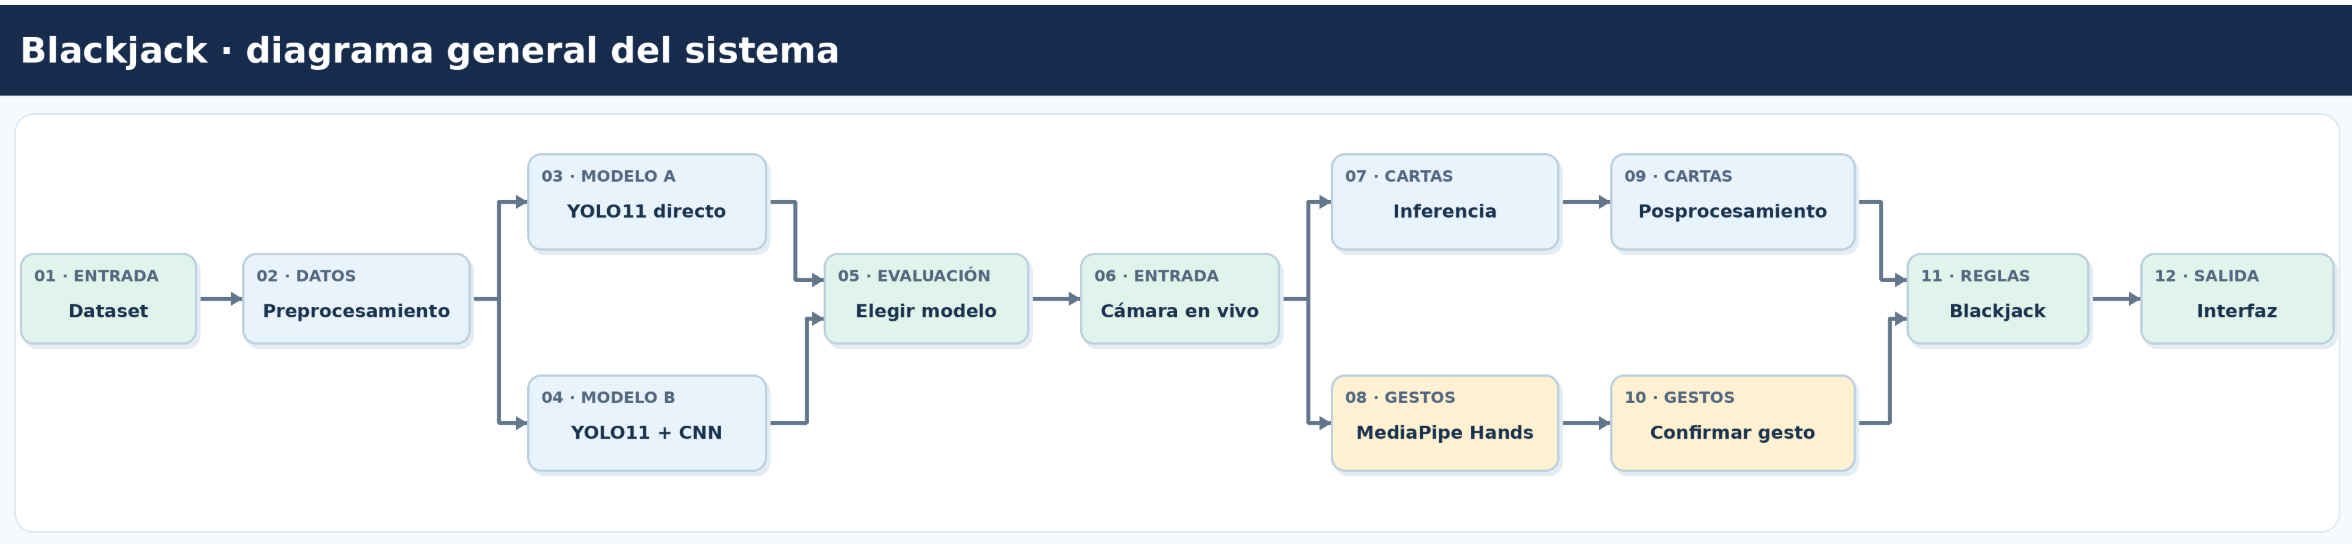
\includegraphics[width=\textwidth]{figuras/arquitectura.png}
\caption{Arquitectura del sistema. Se entrenan los modelos A y B y se elige uno (bloques 01--05); cada cuadro de la cámara pasa por la inferencia de cartas y por MediaPipe, y ambas salidas alimentan el motor
de reglas y la interfaz (bloques 06--12).}
\label{fig:arquitectura}
\end{figure*}

La Fig.~\ref{fig:arquitectura} muestra la arquitectura general del sistema propuesto. El desarrollo se divide en dos etapas principales. La primera corresponde al entrenamiento y evaluación de modelos para la detección y reconocimiento del índice de las cartas. La segunda etapa corresponde a la operación en tiempo real, donde el modelo seleccionado se integra con módulos de captura de video, reconocimiento de gestos, lógica de Blackjack e interfaz de usuario.

\subsection{Datos}
Los datos utilizados provienen de tres datasets diferentes: uno sintético, uno público y otro propio.

\textbf{Sintético.} 10.100 imágenes de (720$\times$720 (7.070 / 2.020 / 1.010) derivadas del dataset \emph{Playing
Cards} de Roboflow \cite{roboflowcards}: cartas generadas y pegadas sobre fondos texturados, con las etiquetas
reducidas a 13 valores (A) o a una única clase (Esquina de carta) (B). Para la CNN de (B) se recortaron las cajas con un margen del 10\%
(28.280 / 8.080 / 4.040 recortes).

\textbf{Real público.} 98 fotos de 416$\times$416 (69 / 18 / 11) de \cite{kostadinov2024}: un solo palo (corazones) y
un mazo con índices en las cuatro esquinas.

\textbf{Real propio.} Para el escenario de la demo se grabaron sesiones con la cámara del juego (un celular cenital)
y se extrajeron 130 cuadros (79 / 21 / 30) que se pre-etiquetaron con el modelo (A) y se corrigieron a mano: 1.688
esquinas, con un gran número de cartas superpuestas. Los conjuntos se separaron por sesión, para evitar el dataleakage a causa de cuadros similares
en los datasets entrenamiento y prueba.

\subsection{Modelos}
El modelo de detección final utilizado surgió de la comparación entre dos estrategia:

\textbf{A (una etapa):} se utilizó YOLO11s \cite{ultralytics2024,khanam2024}, inicializado con pesos preentrenados sobre COCO y adaptado para detectar y clasificar directamente los índices de las cartas en 13 rangos. El modelo fue entrenado durante 50 épocas con imágenes de entrada de 640$\times$640 píxeles. Se seleccionó YOLO11s por ofrecer un compromiso adecuado entre capacidad de detección y costo computacional, además de su integración con herramientas de seguimiento utilizadas posteriormente en el procesamiento de video.


\textbf{B (dos etapas):} de manera análoga, se entrenó YOLO11s para la detección de una única clase, correspondiente a los índices localizados en las esquinas de las cartas. Cada región detectada es recortada y enviada a una ResNet-18 \cite{he2016}, inicializada con pesos preentrenados sobre ImageNet y adaptada para clasificar los recortes entre los 13 rangos posibles. Las imágenes de entrada al clasificador se redimensionan a \(96 \times 96\) píxeles. 

La hipótesis que impulsó el desarrollo de ambas arquitecturas fue la idea de que separar ``dónde'' de ``qué'' facilita la tarea de identificación de las cartas. Una estrategia conceptualmente similar fue evaluada por Chung y Ravella \cite{chung2024}, quienes desacoplaron la localización de las cartas de su clasificación y obtuvieron mejores resultados que con un YOLOv8 entrenado para resolver ambas tareas conjuntamente.

\subsection{Entrenamiento}

Los modelos de ambas arquitecturas se entrenaron utilizando las mismas particiones de entrenamiento, validación y prueba del dataset sintético, con el objetivo de mantener una comparación consistente. El conjunto de prueba se reservó exclusivamente para la evaluación final de los modelos.

\textbf{Detectores YOLO.} Tanto el detector de 13 clases de la arquitectura A como el detector de una única clase de la arquitectura B se inicializaron a partir de pesos preentrenados de YOLO11s. Ambos modelos se entrenaron durante un máximo de 50 épocas, con imágenes de entrada de $640\times640$ píxeles y un tamaño de lote de 16. Se utilizó la selección automática del optimizador provista por Ultralytics y \textit{early stopping} con una paciencia de 15 épocas. Durante el entrenamiento se almacenó el \textit{checkpoint} correspondiente al mejor modelo para su posterior evaluación.

\textbf{Clasificador ResNet-18.} Para la segunda etapa de la arquitectura B se utilizó una ResNet-18 inicializada con pesos preentrenados sobre ImageNet. La última fully connected se reemplazó por una capa de 13 salidas y se ajustaron todos los parámetros de la red sobre los recortes de los índices. El entrenamiento se realizó con lotes de 128 imágenes durante un máximo de 12 épocas.

Como función de pérdida se utilizó Cross-Entropy con \textit{label smoothing} de 0,05. La optimización se realizó mediante AdamW, con una tasa de aprendizaje máxima de $10^{-3}$, \textit{weight decay} de $10^{-4}$ y un planificador OneCycleLR. El mejor modelo se seleccionó según la exactitud sobre el conjunto de validación y se aplicó \textit{early stopping} después de cuatro épocas consecutivas sin mejora.

Durante el entrenamiento del clasificador se aplicaron aumentos de datos consistentes en pequeñas transformaciones afines (rotación de hasta $15^\circ$, traslación y cambios de escala), modificaciones de brillo, contraste, saturación y tono, y desenfoque gaussiano aleatorio. No se utilizaron volteos, ya que una imagen espejada del índice de una carta no representa una configuración válida. Para validación y prueba únicamente se realizó el redimensionamiento y la normalización correspondiente a ImageNet.


\textbf{\textit{Fine-tuning} utilizando imágenes reales:} partiendo de los modelos entrenados sobre el dataset sintético, se realizó una segunda etapa de entrenamiento incorporando imágenes reales. Se llevaron a cabo dos experimentos independientes: uno utilizando el dataset real público (\emph{ft}) y otro utilizando el dataset real propio (\emph{propio}). En cada época, las imágenes reales de entrenamiento se combinaron con una muestra de 400 imágenes del dataset sintético, repitiendo cinco veces las imágenes reales para aumentar su representación durante el ajuste. La selección del mejor modelo se realizó utilizando exclusivamente el conjunto de validación real correspondiente, manteniendo el conjunto de test real reservado para la evaluación final.

\subsection{De esquinas a cartas y a la partida}
La integración del sistema en video en vivo introdujo varios desafíos adicionales. Entre ellos se encuentran la asignación precisa de las cartas a cada jugador, el seguimiento temporal de las cartas ante posibles oclusiones y movimientos, y la identificación robusta de los gestos utilizados durante la partida.

\textbf{Emparejamiento.} Cada carta suele generar dos detecciones, correspondientes a dos de sus esquinas opuestas. Para determinar cuáles pertenecen a una misma carta, se comparan la distancia entre sus centroides y la orientación de la diagonal que los une. Dos esquinas se consideran compatibles cuando la distancia entre sus centros, normalizada por el tamaño de las detecciones, se encuentra entre $3{,}3$ y $4{,}8$, y la línea que las une presenta un ángulo próximo a $50^\circ$ para cartas verticales o a $140^\circ$ para cartas giradas. Estos umbrales se calibraron empíricamente a partir de las esquinas etiquetadas en el dataset propio.

Entre los pares compatibles se priorizan aquellos con mejor ajuste geométrico, evitando asignar una misma esquina a más de una carta. Si una esquina no puede emparejarse, se conserva igualmente como una carta individual, asumiendo que su esquina opuesta puede encontrarse ocluida. Finalmente, se eliminan detecciones redundantes. Por ejemplo, si el modelo detecta más de una vez una misma esquina, se conserva únicamente una de las detecciones. Asimismo, una detección adicional situada dentro de una carta ya reconstruida se descarta cuando su geometría no resulta compatible con la existencia de una carta diferente.

\textbf{Seguimiento.} Para reducir las fluctuaciones entre cuadros consecutivos se utiliza ByteTrack \cite{zhang2022bytetrack}, que asigna un identificador persistente (\emph{track ID}) a cada esquina detectada. Para cada identificador, el valor de la carta se estabiliza mediante una votación ponderada por confianza sobre las detecciones de los últimos 15 cuadros. Además, si una esquina deja de detectarse temporalmente, su última posición y valor se conservan durante un máximo de 10 cuadros, permitiendo tolerar pérdidas breves producidas por oclusiones, reflejos o desenfoque. Finalmente, la mano mostrada se estabiliza considerando los últimos 15 cuadros y tomando, para cada valor de carta, la mediana de la cantidad de apariciones observadas.

\textbf{Gestos.} Para la interacción del jugador se utiliza MediaPipe Hands \cite{zhang2020mediapipe}, que proporciona 21 puntos de referencia (\emph{landmarks}) por mano. A partir de ellos, la pose se clasifica utilizando cocientes entre las distancias muñeca--punta y muñeca--nudillo de los dedos, lo que permite reducir la dependencia respecto de la escala y orientación de la mano. El gesto de \emph{apuntar}, definido por el índice extendido y sostenido durante al menos 0,5~s, solicita una nueva carta. Por su parte, una \emph{palma abierta}, sostenida durante al menos 1,2~s o acompañada por un desplazamiento, indica que el jugador desea plantarse.

\textbf{Reglas.} La lógica del juego se implementa mediante un motor de estados que distingue las etapas de reparto, turno del jugador, turno de la casa y fin de la partida. La mano estabilizada por el módulo de seguimiento constituye la entrada válida para actualizar el estado del juego. La casa solicita cartas mientras su puntuación sea inferior a 17, y el valor del As se ajusta dinámicamente entre 11 y 1 para evitar superar 21 cuando sea posible. Para evitar que fluctuaciones transitorias en la detección modifiquen el estado de la partida, los cambios en la mano deben persistir durante varios cuadros antes de ser aceptados. Se requieren 5 cuadros estables para cambios esperados y 20 cuando aparecen cartas que no fueron solicitadas. Además, mientras una mano permanece sobre la mesa no se confirma un nuevo cambio de estado.

\subsection{Protocolo de evaluación}

Una detección se considera correctamente localizada cuando presenta una intersección sobre unión (IoU, \emph{Intersection over Union}) mayor o igual a $0{,}5$ con una esquina anotada. Para considerar correcta la detección completa, además debe coincidir el rango predicho con el rango real. Se reportan mAP@0.5, precisión (P), \emph{recall} (R) y F1, junto con la latencia media de inferencia por imagen. Para las métricas basadas en predicciones se utiliza un umbral de confianza de $0{,}5$. La latencia se mide en CPU sobre un AMD Ryzen 7 7840U.

\begin{figure*}[!t]
    \centering
    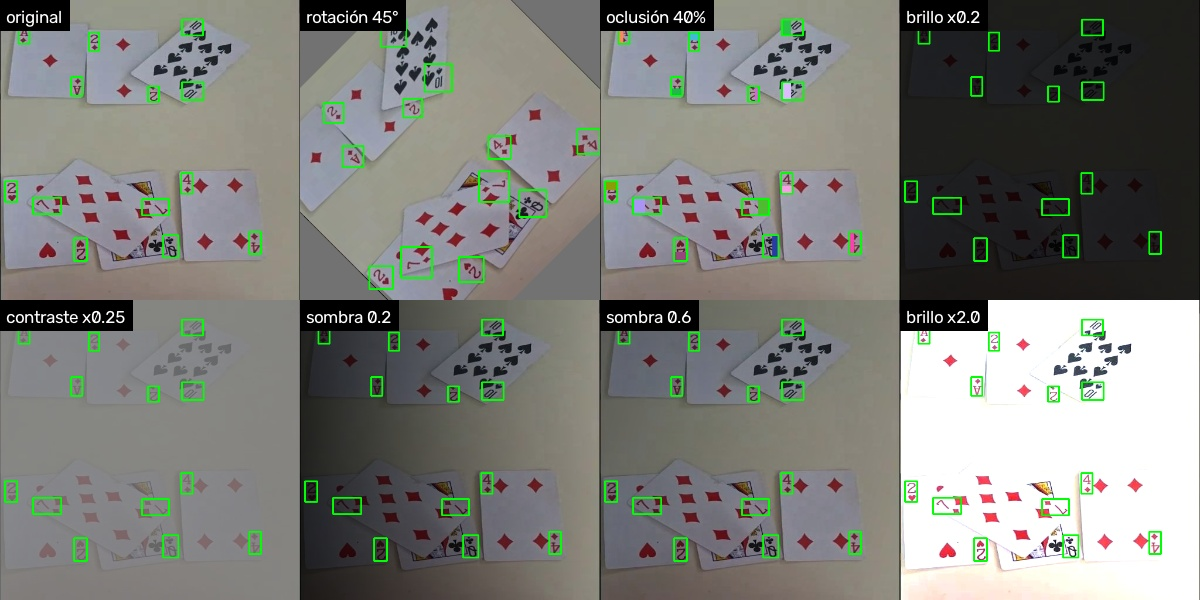
\includegraphics[width=0.86\textwidth]{figuras/perturbaciones.jpg}
    \caption{Ejemplos de las cinco familias de perturbaciones utilizadas para evaluar robustez: rotación, oclusión, brillo, contraste y sombra. Las cajas verdes indican las esquinas anotadas. Cada familia se evalúa en distintos niveles de severidad; en las sombras, el valor indicado corresponde al nivel mínimo de iluminación.}
    \label{fig:perturbaciones}
\end{figure*}



\textbf{Robustez.} La robustez de los modelos se evalúa sobre el conjunto de test propio (30 cuadros, 412 esquinas anotadas) y sobre una muestra fija de 100 imágenes del test sintético. Sobre estas imágenes se aplican cinco familias de perturbaciones visuales (Fig.~\ref{fig:perturbaciones}): rotación, oclusión, variaciones de brillo, variaciones de contraste y sombras. La rotación se realiza alrededor del centro de la imagen, con seis niveles entre $15^\circ$ y $180^\circ$; las anotaciones se transforman junto con la imagen. La oclusión se simula cubriendo cada índice mediante un rectángulo generado desde uno de sus bordes, con seis niveles de severidad entre el 10\% y el 60\%. El brillo se modifica mediante seis factores de ganancia entre $\times 0{,}2$ y $\times 2{,}5$. El contraste se evalúa en cuatro niveles y las sombras se simulan mediante un gradiente de iluminación, también en cuatro niveles de severidad.

Para garantizar una comparación controlada, todos los modelos reciben exactamente las mismas imágenes perturbadas, utilizando una semilla fija para las transformaciones aleatorias. La robustez frente al cambio de fondo se evalúa por separado. Dado que reemplazar el fondo de fotografías reales mediante una máscara de color no produjo composiciones suficientemente confiables, se generaron 30 escenas sintéticas a partir de siete cartas reales recortadas del mazo utilizado en la demostración. Las escenas contienen seis rangos y un total de 244 esquinas anotadas, distribuidas sobre ocho fondos diferentes. Las cartas y sus posiciones se mantienen constantes entre configuraciones, de modo que únicamente varía el fondo.

\textbf{Análisis de errores.} Para caracterizar los errores de detección y clasificación, cada esquina real se asocia con la predicción que presenta la mayor superposición espacial, siempre que su IoU sea mayor o igual a $0{,}5$, independientemente del rango predicho. Esto permite distinguir entre errores de clasificación (la esquina se localiza correctamente pero se asigna un rango incorrecto), falsos negativos (la esquina no es detectada) y falsos positivos (detecciones que no pueden asociarse con ninguna esquina real).

\vspace{4mm}



% =====================================================================================================================
\section{Resultados}

\subsection{Brecha sintético--real y \textit{fine-tuning}}

\begin{table}[!h]
\centering
\caption{Comparación de las arquitecturas A y B en los dominios sintético y reales, antes y después del \textit{fine-tuning}. \emph{ft}: ajuste con el dataset real público; \emph{propio}: ajuste con el dataset propio.}
\label{tab:dominios}
\setlength{\tabcolsep}{3.2pt}
\begin{tabular}{lcccccc}
\toprule
 & \multicolumn{2}{c}{Sintético} & \multicolumn{2}{c}{Real público} & \multicolumn{2}{c}{Real propio} \\
\cmidrule(lr){2-3}\cmidrule(lr){4-5}\cmidrule(lr){6-7}
Modelo & mAP50 & F1 & mAP50 & F1 & mAP50 & F1 \\
\midrule
A base       & 0,995 & 1,00 & 0,68 & 0,72 & 0,86 & 0,78 \\
B base       & 0,995$^\dagger$ & 1,00 & 0,68 & 0,72 & 0,82 & 0,78 \\
A \emph{ft}     & --    & --   & \textbf{0,89} & \textbf{0,89} & 0,86 & 0,78 \\
B \emph{ft}     & --    & --   & 0,77 & 0,78 & 0,90 & 0,83 \\
A \emph{propio} & --    & --   & 0,70 & 0,71 & \textbf{0,98} & \textbf{0,96} \\
B \emph{propio} & --    & --   & 0,75 & 0,73 & 0,94 & 0,93 \\
\midrule
\multicolumn{7}{l}{Latencia (ms/imagen): A 100--114; B 136--143} \\
\bottomrule
\multicolumn{7}{l}{\footnotesize $^\dagger$Detector de B; la CNN alcanza 100\% de exactitud en el test sintético.}
\end{tabular}
\end{table}

La Tabla~\ref{tab:dominios} evidencia una marcada brecha entre el dominio sintético y los escenarios reales. En el test sintético, ambas arquitecturas alcanzan un mAP50 de 0,995 y F1 de 1,00; adicionalmente, la CNN de la arquitectura B obtiene una exactitud del 100\% sobre los recortes sintéticos. Sin embargo, al evaluar los modelos base sobre imágenes reales, el mAP50 disminuye hasta valores comprendidos entre 0,68 y 0,86. Este resultado muestra que un desempeño prácticamente perfecto sobre datos sintéticos no garantiza una generalización equivalente ante cambios de mazo, iluminación, fondo, orientación y condiciones de captura.

El \textit{fine-tuning} con imágenes reales permite reducir esta brecha, aunque su efecto depende fuertemente del dominio utilizado para el ajuste. La arquitectura A ajustada con el dataset real público aumenta su F1 de 0,72 a 0,89 sobre ese mismo dominio, pero mantiene un F1 de 0,78 sobre el escenario propio. De manera análoga, al realizar el ajuste con las 79 imágenes de entrenamiento del dataset propio, A alcanza un mAP50 de 0,98 y un F1 de 0,96 en dicho escenario, mientras que su desempeño sobre el dataset público permanece próximo al del modelo base.

Este comportamiento indica que la adaptación con una cantidad reducida de imágenes representativas del escenario de despliegue resulta más efectiva que utilizar imágenes reales provenientes de otro mazo y otras condiciones de captura. La arquitectura B presenta una transferencia ligeramente mayor entre dominios: al ajustarla con el dataset público, su F1 sobre el escenario propio aumenta de 0,78 a 0,83. Una posible explicación es que parte del ajuste afecta al detector de una única clase, cuya tarea consiste únicamente en localizar índices y no en reconocer directamente su valor. No obstante, esta mejora continúa siendo inferior a la obtenida al incorporar imágenes del escenario objetivo, donde B alcanza un F1 de 0,93.

\textbf{Selección del modelo.} A partir de estos resultados se seleccionó la arquitectura A para la aplicación final. Una vez ajustada con imágenes propias, A obtiene el mejor desempeño en el dominio de despliegue, con mAP50 de 0,98 y F1 de 0,96, frente a 0,94 y 0,93 de B, respectivamente. La diferencia también se observa en el costo computacional: A requiere entre 100 y 114~ms por imagen, mientras que B requiere entre 136 y 143~ms.

Además de la mejora cuantitativa, A presenta una arquitectura más simple para la operación en tiempo real. Cada índice es localizado y clasificado mediante una única inferencia, mientras que B requiere primero ejecutar YOLO para localizarlo y posteriormente procesar cada recorte mediante ResNet-18. Esta segunda estrategia introduce una etapa adicional de cómputo y una posible propagación de errores: una localización imprecisa del detector puede producir un recorte incompleto o descentrado y afectar posteriormente la clasificación. Por lo tanto, dado que la separación entre localización y clasificación no produjo una mejora de precisión que compensara este costo adicional, se optó por A como modelo final por ofrecer el mejor compromiso entre desempeño, latencia y simplicidad de integración.

\subsection{Robustez}

\begin{figure*}[t]
\centering
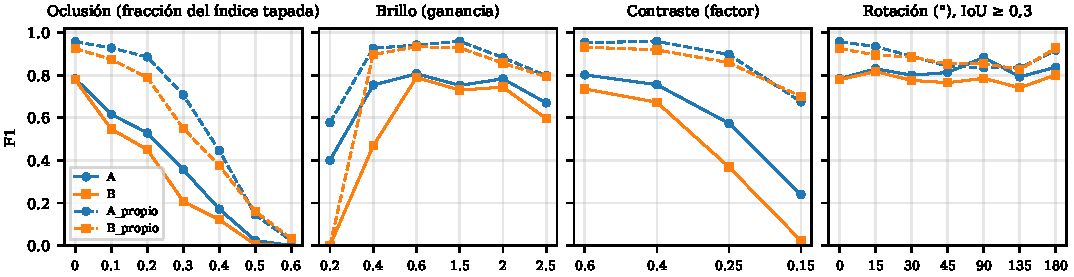
\includegraphics[width=\textwidth]{figuras/robustez.pdf}
\caption{F1 en el test propio en función de la severidad de cada perturbación (trazo lleno: modelos base; trazo
cortado: ajustados con fotos propias). Las rotaciones se miden con IoU $\geq$ 0,3 (ver texto).}
\label{fig:robustez}
\end{figure*}

\begin{table}[!h]
\centering
\caption{F1 medio de cada arquitectura ante las distintas familias de perturbaciones. Cada valor corresponde al promedio sobre los niveles de severidad evaluados. La categoría iluminación agrupa las perturbaciones de brillo, contraste y sombra.}
\label{tab:robustez}
\setlength{\tabcolsep}{4pt}
\begin{tabular}{llcccc}
\toprule
Dominio & Familia & A & B & A \emph{propio} & B \emph{propio} \\
\midrule
\multirow{3}{*}{Real propio} & Rotación & 0,76 & 0,72 & \textbf{0,81} & 0,80 \\
 & Oclusión    & 0,28 & 0,22 & \textbf{0,52} & 0,46 \\
 & Iluminación & 0,69 & 0,58 & \textbf{0,88} & 0,82 \\
\midrule
\multirow{3}{*}{Sintético} & Rotación & 0,74 & 0,72 & 0,74 & 0,71 \\
 & Oclusión    & \textbf{0,74} & 0,63 & 0,72 & 0,61 \\
 & Iluminación & \textbf{0,99} & 0,98 & 0,99 & 0,98 \\
\bottomrule
\end{tabular}
\end{table}

\begin{table}[!h]
\centering
\caption{F1 sobre escenas compuestas manteniendo las mismas siete cartas y posiciones y variando únicamente el fondo.}
\label{tab:fondo}
\setlength{\tabcolsep}{2.6pt}
\begin{tabular}{lcccccccc}
\toprule
 & Mad. & Verde & Osc. & Blanco & Text. & Desor. & Ruido & Márm. \\
\midrule
A               & 0,99 & 1,00 & 1,00 & 0,99 & 1,00 & 1,00 & 0,99 & 1,00 \\
B               & 0,98 & 0,99 & 0,99 & \textbf{0,90} & 0,97 & 0,97 & 0,98 & 0,99 \\
A \emph{propio} & 0,99 & 0,99 & 0,99 & 0,98 & 0,99 & 0,99 & 0,99 & 0,99 \\
B \emph{propio} & 1,00 & 1,00 & 1,00 & 1,00 & 1,00 & 1,00 & 0,99 & 1,00 \\
\bottomrule
\end{tabular}
\end{table}

La Tabla~\ref{tab:robustez} resume el efecto de las distintas familias de perturbaciones, mientras que la Fig.~\ref{fig:robustez} muestra la evolución del F1 al aumentar su severidad. En conjunto, los experimentos muestran tres comportamientos principales: la oclusión constituye la perturbación más crítica, las alteraciones de iluminación afectan considerablemente más al dominio real que al sintético y las variaciones de fondo tienen un efecto reducido.

\textbf{Oclusión.} La oclusión produce la mayor degradación entre las perturbaciones evaluadas. En el dominio sintético, A mantiene un F1 de 0,95 con un 30\% del índice ocluido y desciende a 0,52 al alcanzar el 50\%. La degradación aparece considerablemente antes en imágenes reales: A base cae de 0,78 a 0,62 con apenas un 10\% de oclusión y a 0,36 con un 30\%. El \textit{fine-tuning} con imágenes propias aumenta notablemente esta tolerancia, alcanzando F1 de 0,93 y 0,89 para oclusiones del 10\% y 20\%, respectivamente. Este resultado motivó decisiones posteriores del sistema, como conservar esquinas no emparejadas como cartas válidas y mantener temporalmente detecciones perdidas mediante el módulo de seguimiento.

\textbf{Iluminación.} Se observa una diferencia marcada entre los dominios sintético y real. Sobre imágenes sintéticas, las perturbaciones de iluminación apenas modifican el desempeño medio, que permanece por encima de 0,98. En cambio, las imágenes reales presentan una sensibilidad considerable a condiciones extremas de subexposición y bajo contraste. Con brillo reducido a $\times0,2$, A base alcanza F1 de 0,40 y B deja de producir detecciones correctas; con contraste $\times0,15$, A base desciende a 0,24. El ajuste con imágenes propias mejora especialmente a A, cuyo F1 medio frente a perturbaciones de iluminación aumenta de 0,69 a 0,88. Esto sugiere que parte de la brecha sintético/real observada anteriormente está asociada a la representación de las condiciones de iluminación del escenario objetivo.

\textbf{Rotación.} La evaluación de rotaciones requiere considerar el efecto de la métrica de localización. Al utilizar IoU $\geq 0,5$, se observa una caída pronunciada a $45^\circ$ incluso sobre imágenes sintéticas. Sin embargo, parte de esta disminución se debe a que las cajas anotadas y predichas permanecen alineadas con los ejes, por lo que la caja envolvente de un índice rotado aumenta de tamaño y reduce artificialmente su IoU. Al relajar únicamente para este análisis el umbral a IoU $\geq 0,3$, A alcanza F1 de 0,98 a $45^\circ$ y valores próximos a 1,00 para rotaciones mayores en el dominio sintético. En el dominio real persiste una degradación moderada, lo que indica que no todo el efecto puede atribuirse a la métrica.

\textbf{Fondo.} A diferencia de las perturbaciones anteriores, el cambio de fondo presenta un impacto mínimo. En las escenas controladas de la Tabla~\ref{tab:fondo}, A mantiene F1 $\geq 0,99$ en los ocho fondos evaluados. El caso de mayor degradación corresponde a B base sobre fondo blanco, con F1 de 0,90. Dado que las cartas y sus posiciones permanecen constantes entre escenas, estos resultados indican que el fondo, por sí solo, no constituye una fuente importante de error para el sistema.

\subsection{Análisis de errores}

\begin{table}[!h]
\centering
\caption{Errores por esquina en el test propio (412 esquinas reales).}
\label{tab:errores}
\setlength{\tabcolsep}{3pt}
\begin{tabular}{lccccl}
\toprule
 & Bien & \begin{tabular}[c]{@{}c@{}}Valor\\ equivocado\end{tabular} & \begin{tabular}[c]{@{}c@{}}No\\ detectada\end{tabular}
 & \begin{tabular}[c]{@{}c@{}}Falsos\\ positivos\end{tabular} & \begin{tabular}[c]{@{}l@{}}Confusión más\\ frecuente\end{tabular} \\
\midrule
A               & 66,3\% & 1,7\% & \textbf{32,0\%} & 5  & 8$\to$6 (5) \\
B               & 64,1\% & 0,2\% & \textbf{35,7\%} & 1  & A$\to$4 (1) \\
A \emph{propio} & \textbf{95,6\%} & \textbf{0\%} & 4,4\% & 17 & ninguna \\
B \emph{propio} & 93,0\% & 2,2\% & 4,9\% & 24 & 5$\to$3 (5) \\
\bottomrule
\end{tabular}
\end{table}

La Tabla~\ref{tab:errores} permite identificar el origen de los errores observados en el test propio. En los modelos base, el principal problema no es la asignación incorrecta del valor, sino la ausencia de detección: A no detecta el 32,0\% de las esquinas y B el 35,7\%, mientras que los errores de clasificación representan únicamente el 1,7\% y 0,2\%, respectivamente.

El \textit{fine-tuning} con imágenes propias modifica sustancialmente este comportamiento. En A \emph{propio}, las esquinas no detectadas disminuyen del 32,0\% al 4,4\% y no se observan errores de clasificación, aunque aumenta el número de falsos positivos de 5 a 17. B presenta una tendencia similar, reduciendo las esquinas no detectadas al 4,9\%, pero conserva un 2,2\% de errores de clasificación y genera 24 falsos positivos.

Estos resultados refuerzan lo observado en los experimentos de robustez: el principal desafío del sistema se encuentra en la localización de los índices bajo condiciones reales, más que en distinguir su rango una vez localizados. En particular, para A \emph{propio}, el rango 8 concentra 13 de las 18 esquinas no detectadas, lo que sugiere que parte del error residual se encuentra concentrado en casos específicos y no distribuido uniformemente entre las clases.
\subsection{Sistema completo}

\begin{figure}[!h]
\centering
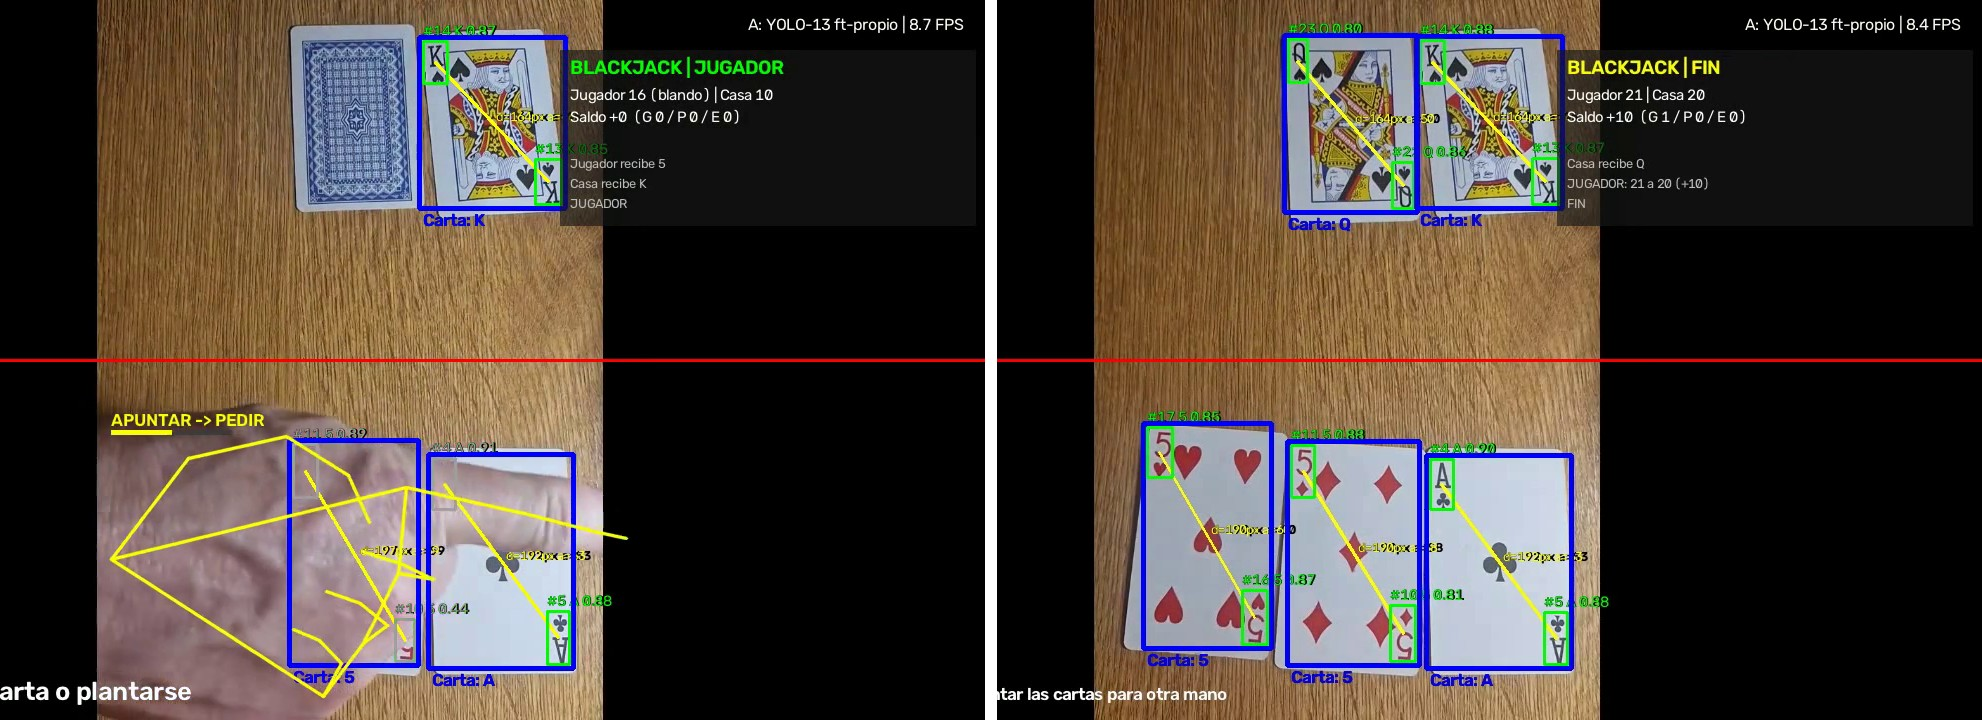
\includegraphics[width=\columnwidth]{figuras/aplicacion.jpg}
\caption{Ejemplo de una partida real procesada por el sistema. Izquierda: el gesto de \emph{apuntar} solicita una nueva carta. Derecha: estado final de la partida, con las cartas detectadas, los puntajes y los eventos registrados por la aplicación.}
\label{fig:aplicacion}
\end{figure}

Se evaluó el comportamiento del sistema una vez integrados sus distintos componentes. En particular, se analizó cuantitativamente la estabilidad del seguimiento temporal y la robustez del reconocimiento de gestos, y se realizó una validación funcional del prototipo completo mediante partidas reales de Blackjack.

\textbf{Seguimiento.} Para evaluar el aporte del seguimiento temporal se utilizaron videos con movimiento de cámara simulado. La incorporación del módulo de seguimiento aumentó la proporción de cuadros en los que se mostró correctamente la mano del 50,5\% al 76,2\%. Además, en intervalos de 10~s, la cantidad de cambios en la mano mostrada se redujo de 47 a 4. Estos resultados muestran que la combinación del seguimiento de las esquinas, la memoria temporal y la estabilización de la mano reduce considerablemente las fluctuaciones producidas por pérdidas momentáneas de detecciones.

\textbf{Gestos.} El reconocimiento de gestos se evaluó sobre imágenes reales de HaGRID \cite{kapitanov2024hagrid}. La estrategia propuesta alcanza un \emph{recall} de 0,80 para el gesto de \emph{apuntar} y de 0,89 para \emph{palma}, manteniendo estos valores al rotar las imágenes $90^\circ$ y $180^\circ$. Esta invariancia resulta especialmente relevante para una cámara cenital, donde la orientación de la mano respecto de la imagen puede variar considerablemente. En clips de video, el gesto de \emph{palma} se reconoce correctamente en el 82--87\% de los casos, con un 4,2\% de activaciones falsas.

\textbf{Partidas reales.} Finalmente, se realizó una validación integral del prototipo mediante partidas completas de Blackjack grabadas en el escenario de la aplicación. Los casos evaluados incluyeron distintas situaciones del juego, entre ellas victorias del jugador y de la Casa, el ajuste dinámico del valor del As de 11 a 1 y la presencia de cartas giradas. Al reproducir posteriormente las partidas cuadro a cuadro, el sistema reprodujo correctamente los resultados finales, las cartas detectadas y los gestos registrados durante la ejecución en vivo (Fig.~\ref{fig:aplicacion}).

Estos videos se conservaron además como casos de prueba de regresión para verificar el comportamiento integral del sistema ante futuras modificaciones. Durante su ejecución, el prototipo operó a una velocidad de 7--10 cuadros por segundo en CPU, permitiendo la detección de cartas, el seguimiento temporal, el reconocimiento de gestos y la actualización de la lógica del juego en tiempo real.

% =====================================================================================================================
\section{Conclusiones}

Los experimentos realizados permiten extraer conclusiones tanto sobre el desempeño del modelo de visión como sobre la robustez y el funcionamiento del sistema completo en condiciones reales:

\begin{enumerate}
\item El rendimiento en el dataset sintético (mAP50 0,995) no anticipa el rendimiento real (0,68--0,86): evaluar con
fotos del escenario de uso es imprescindible.
\item El \textit{fine-tuning} con datos reales mejora sobre todo el dominio con el que se hace: 79 cuadros del escenario
propio llevaron el recall de A de 0,66 a 0,96, mientras que fotos de otro mazo no mejoraron a A y solo mejoraron
parcialmente a B (F1 de 0,78 a 0,83), a través de su detector.
\item En el escenario de uso, el detector de una etapa (A) superó al de dos (B) en exactitud y latencia: el contexto que ve el detector
ayuda a distinguir valores similares, mientras que la CNN de B clasifica un recorte aislado.
\item En datos reales el error dominante no es confundir valores sino no encontrar la esquina; la oclusión es la
perturbación más dañina y la iluminación pesa mucho más que en los datos sintéticos.
\item El fondo casi no influye, y la caída aparente ante rotaciones oblicuas se explica en gran parte por la métrica
(IoU de cajas alineadas).
\item La lógica de posprocesamiento —emparejamiento geométrico, supresión de detecciones superpuestas mediante NMS agnóstico a la clase, seguimiento temporal y congelamiento del estado de la mesa ante oclusiones por las manos— fue decisiva para pasar de detecciones independientes por fotograma a una representación consistente de las manos en partidas reales.
\item Para gestos con cámara cenital, reglas invariantes a la rotación sobre los puntos de MediaPipe funcionan donde el
clasificador preentrenado falla.
\end{enumerate}
\textbf{Trabajo futuro:}
\begin{itemize}
    \item\ Reconocer el palo (permitiría detectar cartas duplicadas, imposibles con un solo mazo),
    \item\ Entrenar con la cámara en ambas orientaciones, más mesas e iluminaciones en el test propio.
    \item\ Ampliar la detección y dinámica a varios jugadores.
\end{itemize}


\bibliographystyle{IEEEtran}
\bibliography{referencias}

\end{document}
